% !TEX root = main.tex
\section{PLLの基本構成と分数分周比PLLの課題}
\label{sec:pll-basics}

\subsection{PLLの基本構成とノイズ増幅}

一般的なPLLは，入力とフィードバックの位相差を比較する位相比較器(Phase Detector, PD)，PDの出力をアナログに変換するチャージポンプ(Charge Pump, CP)，ノイズを除去するループフィルタ(Loop Filter, LF)，CPの出力に応じた周波数を出力する電圧制御発振器(Voltage-Controlled Oscillator, VCO)，そしてVCOの出力を基準周波数まで分周して位相検出器に戻す分周器(Divider，分周比 $N$)から構成される．図\ref{fig:pll-linear-model}は一般的なPLLのモデルを表す．ただしCPは，PDに含めて表記している．これは，PDとCPが連携して「入力された位相差 $\Delta\phi$ に応じた電流を出力する」という一連の動作を担っており，両者が生み出す雑音はどちらも出力電流に現れるため，両者を区別する意味がないからである．

このようなPLLの動作は次のように進行する．基準信号 $f_\text{REF}$ と，出力を $N$ 分周した信号の位相差をPDが検出し，CPが出力する．その誤差信号をLFで整形し，VCOの発振周波数を制御することで，最終的に出力周波数は $f_\text{OUT} = N f_\text{REF}$ にロックする．

\begin{figure}[H]
  \centering
  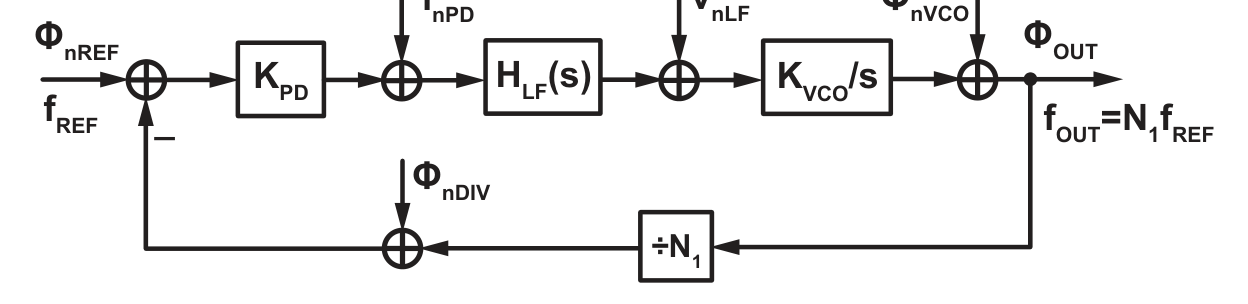
\includegraphics[keepaspectratio,width=0.85\columnwidth]{fig/fig_2_1.png}
  \caption{PLLの線形モデル(本文Fig.\,2.1，\cite{osada_thesis})．ループの各所(基準・PD・ループフィルタ・VCO・分周器)にそれぞれ固有の雑音源がぶら下がる形でモデル化できる．}
  \label{fig:pll-linear-model}
\end{figure}

PLLは負帰還系であるため，図\ref{fig:feedback-noise-amp}(a)に示すように単純化して記述できる．帰還利得を $\beta$ ，フィードフォワード利得を $A(s)$ とすると，ループ利得が十分大きい帯域($|\beta A(s)| \gg 1$，VCOの積分特性とPLLの追従動作により，通常はこの条件が満たされるように設計される)では，閉ループゲインは $\frac{A(s)}{1 + \beta A(s)} \approx \frac{1}{\beta}$ と近似できる．つまり，ループの入力側に入る雑音は，出力時に $1/\beta$ 倍に増幅されて現れるということである．従来型のPLLでは帰還経路に分周比 $N$ の分周器を用いるため $\beta = 1/N$ となり，基準発振器やPDの雑音，そして後述する分周器由来の(量子化)雑音は，すべて \textbf{$N$ 倍}に増幅されて出力に現れることになる(図\ref{fig:feedback-noise-amp}(b))．例えば基準周波数100\,MHzから2.4\,GHzを生成する場合，$N=24$ であるから $20\log_{10}(24) \approx 27.6$\,dBもの増幅を受ける．これが，分数分周比PLLを設計する上での根本的な制約となる．

\begin{figure}[H]
  \centering
  
\includegraphics[keepaspectratio,width=0.85\columnwidth]{fig/fig_3_1.png}
  \caption{負帰還系における入力換算雑音の増幅(本文Fig.\,3.1，\cite{osada_thesis})．(a)一般の負帰還系では入力側雑音は $1/\beta$ 倍される．(b)帰還を「割り算」(分周器，$\beta=1/N$)ではなく「引き算」(ミキサ，$\beta=1$)で実現すれば，雑音は増幅されない．それについては後述．}
  \label{fig:feedback-noise-amp}
\end{figure}

\subsection{分数分周比PLLにおける量子化雑音とフラクショナルスパー}

整数分周比のPLLに対し，出力周波数を基準周波数の小数倍に設定できる分数分周比(Fractional-$N$)PLLは，より細かい周波数分解能を実現できるため広く用いられている．分数分周は，マルチモジュラス分周器(Multi-Modulus Divider, MMD)の分周比を時間的に変化させ，その平均値として目的の小数分周比を実現する(例えば $\div 2.25$ を $2,3,2,2,\dots$ の繰り返しで近似する)．しかし瞬間の分周比は整数値をとり，その値が周期的に切り替わるため，位相誤差が常に変動する．これが\textbf{量子化雑音}であり，そのパターンが周期的だと鋭いスパー(フラクショナルスパー)として現れる．

この量子化雑音は，$\Delta\Sigma$変調器(Delta Sigma Modulator, DSM)によって高域へ押しやる「ノイズシェーピング」によってある程度緩和できる．これは，PLL自体がLPF特性を持つためである．しかし，それでも前述の閉ループゲイン $1/\beta = N$ による増幅を免れることはできない．結果として，分数分周比PLLは整数分周比PLLに比べ，量子化雑音の分だけジッタ性能が大きく悪化するという問題を抱えている(図\ref{fig:frac-pn})．

\begin{figure}[H]
  \centering
  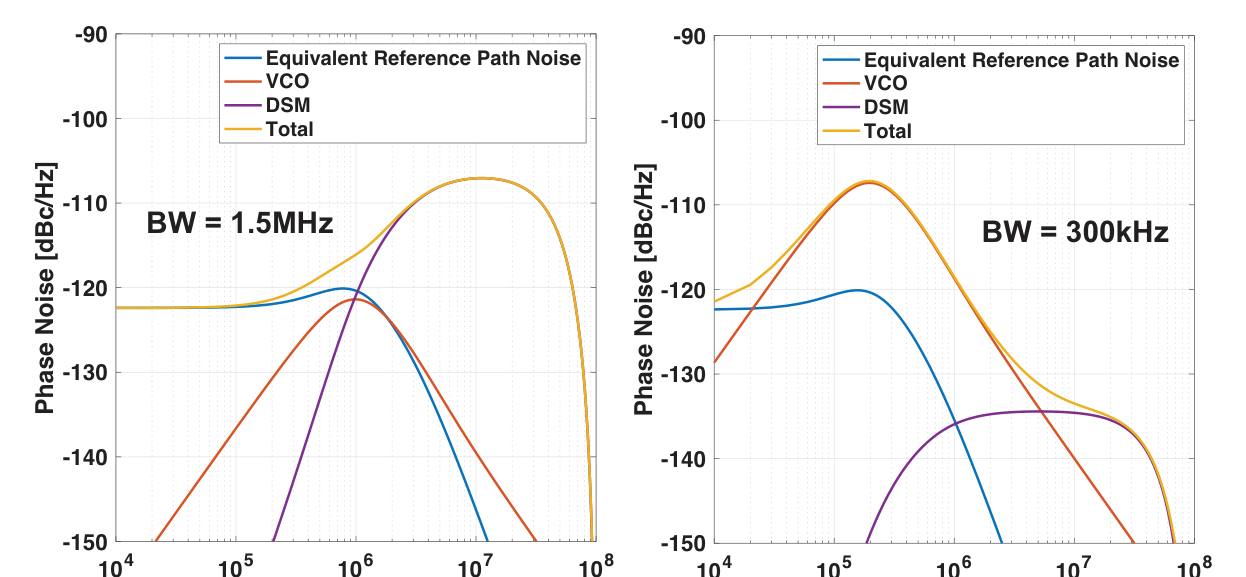
\includegraphics[keepaspectratio,width=0.85\columnwidth]{fig/fig_2_9.png}
  \caption{分数分周比PLLの位相雑音(本文Fig.\,2.9，\cite{osada_thesis})．量子化雑音が上乗せされ，帯域幅が1.5\,MHzでは高周波帯で量子化雑音が支配的になることが示されている．なお，狭帯域にしてもVCO雑音が増えるため根本解決にはならない．}
  \label{fig:frac-pn}
\end{figure}

\subsection{ノイズ増幅を回避する方法}

この量子化雑音増幅の問題に対し，近年注目されているアプローチの一つが，分周器を高調波ミキサ(Harmonic Mixer, HM)による周波数の「引き算」に置き換える方法である．ミキサによってHM出力 $f_\text{HM} = f_\text{OUT} - k f_\text{LO}$($k$ は高調波次数)を生成し，この信号を基準信号と比較する構成にする(ロック時には $f_\text{HM}=f_\text{REF}$ となる)．この時，除算は行われないため，閉ループゲインは $\beta \approx 1$(ユニティ)となり，量子化雑音は増幅されない．したがって，分数分周比PLLの課題である量子化雑音の増幅を回避できる．

なお，$k$倍せず直接$f_\text{HM} = f_\text{OUT} - f_\text{LO}$とすると，$f_\text{REF}$ は小さいため，$f_\text{OUT}$ と $f_\text{LO}$ が非常に近い周波数となる．この場合，その2つが相互に影響しあって新たなノイズを生み出すリスクが生じる．$k$倍することで，相互に影響する高調波成分を非常に弱めることができるため，このような構成が採用される．
